%This is a very basic  BE PROJECT PRELIMINARY template.

%############################################# 
%#########Author :  PROJECT###########
%#########COMPUTER ENGINEERING############


\documentclass[oneside,a4paper,12pt]{report}
%\usepackage{showframe}
%\hoffset = 8.9436619718309859154929577464789pt
%\voffset = 13.028169014084507042253521126761pt

\fancypagestyle{plain}{%
  \fancyhf{}
  \fancyfoot[CE]{College_Name, Department of Computer Engineering 2015}
  \fancyfoot[RE]{\thepage}
}
\pagestyle{fancy}
\fancyhead{}
\renewcommand{\headrulewidth}{0pt}
\footskip = 0.625in
\cfoot{}
\rfoot{}

\usepackage[]{hyperref}
\usepackage{tikz}
\usetikzlibrary{arrows,shapes,snakes,automata,backgrounds,petri}

\usepackage{tabularx}

\usepackage[nottoc,notlot,notlof,numbib]{tocbibind}
\usepackage[titletoc]{appendix}
\usepackage{titletoc}
\renewcommand{\appendixname}{Annexure}
\renewcommand{\bibname}{References}

\setcounter{secnumdepth}{5}

\usepackage{float}
\usepackage{subcaption}
\usepackage{multirow}

%\usepackage[ruled,vlined]{algorithm2e}

\begin{document}

\setlength{\parindent}{0mm}
\begin{center}
{\bfseries SAVITRIBAI PHULE PUNE UNIVERSITY \\}
 \vspace*{1\baselineskip}
{\bfseries A PRELIMINARY PROJECT REPORT ON \\}
 \vspace*{2\baselineskip}
{\bfseries \fontsize{16}{12} \selectfont Physical Web with Vending Machine \\ \vspace*{2\baselineskip}}
{\fontsize{12}{12} \selectfont SUBMITTED TOWARDS THE
 \\PARTIAL FULFILLMENT OF THE REQUIREMENTS OF \\

\vspace*{2\baselineskip}}
{\bfseries \fontsize{14}{12} \selectfont BACHELOR OF ENGINEERING (Computer
Engineering) \\
\vspace*{1\baselineskip}} 
{\bfseries \fontsize{14}{12} \selectfont BY \\ 
\vspace*{1\baselineskip}} 
Student Name: Sejal Khatri \hspace{25 mm} Exam No: B120054336\\
Student Name: Amruta Ranade \hspace{25 mm} Exam No:  B120054223  \\
Student Name: Kevin Kaul\hspace{25 mm} Exam No: B120054333  \\
\vspace*{2\baselineskip}
{\bfseries \fontsize{14}{12} \selectfont Under The Guidance of \\  
\vspace*{2\baselineskip}} 
Prof. A.R.Deshpande\\

\includegraphics[width=100pt]{collegelogo.png} \\
{\bfseries \fontsize{14}{12} \selectfont DEPARTMENT OF COMPUTER ENGINEERING \\
Pune Institute of Computer Technology \\
PICT,Dhankawadi,Pune-411043.
}
\end{center}

\newpage



\begin{figure}[ht]
\centering

\includegraphics[width=100pt]{collegelogo.png}
\end{figure}


{\bfseries \fontsize{14}{12} \selectfont \centerline{Pune Institute of Computer Technology}
\centerline{DEPARTMENT OF COMPUTER ENGINEERING}
\vspace*{3\baselineskip}} 


{\bfseries \fontsize{16}{12} \selectfont \centerline{CERTIFICATE} 
\vspace*{3\baselineskip}} 

\centerline{This is to certify that the Project Entitled}
\vspace*{1\baselineskip} 


{\bfseries \fontsize{14}{12} \selectfont \centerline{ Physical Web with Vending machine.}
\vspace*{1\baselineskip}}

\centerline{Submitted by}
\vspace*{1\baselineskip} 
\centerline{Sejal Khatri  \hspace{25 mm} Exam No:B120054336} 
\centerline{Amruta Ranade \hspace{25 mm} Exam No:B120054223  } 
\centerline{Kevin Kaul \hspace{25 mm} Exam No:B120054333 }
\vspace*{1\baselineskip} 
is a bonafide work carried out by Students under the supervision of Prof.A.R.Deshpande and it
is submitted towards the partial fulfillment of the requirement of Bachelor of Engineering (Computer Engineering) Project.\\\\\\

\bgroup
\def\arraystretch{0.7}
\begin{tabular}{c c }
Prof. A.R.Deshpande &  \hspace{50 mm} Prof. Rajesh Ingle \\								
Internal Guide   &  \hspace{50 mm} H.O.D \\
Dept. of Computer Engg.  &	\hspace{50 mm}Dept. of Computer Engg.  \\
\end{tabular}
%}



\newpage

%\pictcertificate{TITLE OF BE PROJECT}{Student Name}{Exam Seat No}{Guide Name}
\setcounter{page}{0}
\frontmatter
\cfoot{PICT, Department of Computer Engineering 2016}
\rfoot{\thepage}
\pagenumbering{Roman}
%\pictack{Physical Web with Vending Machine}{Prof.A.R.Deshpande}

		
{  \newpage {\bfseries \fontsize{14}{12} \selectfont \centerline{Abstract} 
\vspace*{2\baselineskip}} \setlength{\parindent}{11mm} }
{ \setlength{\parindent}{0mm} }
 A vending machine is a machine that dispenses items such as snacks, bever-
ages to customers automatically, after the customer inserts currency or credit
into the machine. But nowadays paying in cash has become a difficulty and cannot be fulfilled every time.Therefore we provide a platform for the vending machine functionalitiesand management to be handled by cloud using Internet of things.With this approach Online payment for vending machines can be made possible and the
stock record is maintained on the cloud for dynamically updating the vendor.
In addition to which the users are notified about the presence of the vending
machine using Web Bluetooth API.


{  \newpage {\bfseries \fontsize{14}{12} \selectfont \centerline{Acknowledgments} 
\vspace*{2\baselineskip}} \setlength{\parindent}{11mm} }
{ \setlength{\parindent}{0mm} }

\textit{It gives us great pleasure in presenting the preliminary project report 
on {\bfseries \fontsize{12}{12} \selectfont `Physical Web with Vending machine'}.}
\vspace*{1.5\baselineskip}

 \textit{We would like to take this opportunity to thank our internal guide
 \textbf{Prof. A.R.Deshpande} for giving us all the help and guidance we needed. We are really grateful to them for their kind support. Their valuable suggestions were very helpful.} \vspace*{1.5\baselineskip}

 \textit{We are also grateful to \textbf{Prof. Rajesh Ingle}, Head of Computer
 Engineering Department, PICT for his indispensable
 support, suggestions.}
\vspace*{1.5\baselineskip}

\textit{In the end our special thanks to \textbf{Mr. Anuj Deshpande} for
providing various resources such as  laboratory with all needed software platforms,
continuous Internet connection, for Our Project.}
\vspace*{3\baselineskip} \\
\begin{tabular}{p{8.2cm}c}
&Sejal Khatri\\
&Amruta Ranade\\
&Kevin Kaul\\
&(B.E. Computer Engg.)
%}
\end{tabular}


% \maketitle
\tableofcontents
\listoffigures 
\listoftables



\mainmatter



  \titleformat{\chapter}[display]
{\fontsize{16}{15}\filcenter}
{\vspace*{\fill}
 \bfseries\LARGE\MakeUppercase{\chaptertitlename}~\thechapter}
{1pc}
{\bfseries\LARGE\MakeUppercase}
[\thispagestyle{empty}\vspace*{\fill}\newpage]







\setlength{\parindent}{11mm}
\chapter{Synopsis}

\section{Project Title}
Physical Web with Vending Machine
\section{ Project Option }
Industry sponsored

\section{Internal Guide}
Prof. A.R.Deshpande

\section{ Sponsorship and External Guide} 
Sponsored By : Marvell Pvt.ltd.

\section{Technical Keywords (As per ACM Keywords)}
% {\bfseries Technical Key Words:}      
% \begin{itemize}
%   \item 	Cloud Computing
% \item	Service Composition
% \item	Online Web services
% \end{itemize}
\begin{enumerate}

\item IOT.
\item Cloud Computing.
\item Cloud based storage.
\item Web Application.
\item Web Services.
\item Web based interaction.
\item Web Interfaces.
\end{enumerate}



\section{Problem Statement}
\label{sec:problem}
        To Automate vending machine functionalities for vendors and enabling easy accessibility for users through online payment and establishing a physical interface with the help of beacons. 
\section{Abstract}
A vending machine is a machine that dispenses items such as snacks, bever-
ages to customers automatically, after the customer inserts currency or credit
into the machine. But nowadays paying in cash has become a difficulty and cannot be fulfilled every time.Therefore we provide a platform for the vending machine functionalitiesand management to be handled by cloud using Internet of things.With this approach Online payment for vending machines can be made possible and the
stock record is maintained on the cloud for dynamically updating the vendor.
In addition to which the users are notified about the presence of the vending
machine using Web Bluetooth API.
		    		   

\section{Goals and Objectives}
Project Goal :Presently operating the vending machines is not user-friendly and it is observed to be time consuming as well.Our project goal is to increase the scope and quality of the vending machine services provided to the people. 

Project Objective 1:
People use coins or paper money while operating the vending machines due to which there arises a problem when the user does not seem to have exact change with him.
Performance Measure :
Online (cashless) payments are made available for the users for easy purchase of items.

Project Objective 2:
The vendors are not aware about the stock required in the vending machines when excess usage of the products occur.
Performance Measure :
Vendors are well informed about the stock management of the machine and are also aware of the customers past transactions.

Project Objective 3 :
Finding a vending machine in new locations everytime becomes difficult for people.
Performance Measure :
The users are notified about the presence of the vending machine available in their current location using the Web Bluetooth API.
	
\section{Relevant mathematics associated with the Project}
\label{sec:math}
System Description:\\
 Let S be the solution system ,
	  S = {s , e, X, Y, F, DD, NDD , sc, fc | shmem}\\
            where,    \\   
s = start state {Wi-fi interfacing}\\
e = end state { Product delivered and status recorded}\\
X = Input set\\
Y = Output set\\
Input:(Physical address, user’s choice)	\\ 
Output:(Product requested , suggestions)\\ 
Identify data structures, classes, divide and conquer strategies to exploit distributed/parallel/concurrent processing, constraints. \\
Functions : Fme + Ffriend.\\
Fme = Main functions.\\
Fme = (fin , fout,initiate,detect,connect).\\
Ffriend = inbuilt functions.\\
Ffriend = (fproc , fcloud).\\
Mathematical formulation if possible\\
Non Deterministic Data :Single Physical address.\\
Deterministic Data :Valid input.\\
Success Conditions:Valid input( i.e valid user choice) is given and the desired result is obtained successfully and also proper internet availability.\\
Failure Conditions: Invalid input( i.e invalid user choice)  given and desired result not obtained also internet availability not present.\\


\section{Names of Conferences / Journals where papers can be published}

 Physical Web in Smart Cities - Advances in Wireless and Optical Communications (RTUWO), 2015\\
 On physical web models - Control and Communications (SIBCON), 2016 \\
International Siberian Conference Finite state machine based vending machine – International Journal of VLSI design and communication system 2012.\\


\section{Review of Conference/Journal Papers supporting Project idea}
\label{sec:survey}

   

\section{Plan of Project Execution}

\begin{table}[!htbp]
\begin{center}
%\def\arraystretch{1.5}
\def\arraystretch{1.5}
\begin{tabularx}{\textwidth}{| X | X |}
\hline
Activity	& Planned months\\
\hline
Requirement gathering and feasibility studying        &1 july – 15 Aug\\
\hline
Planning Activities       &16 Aug – 31 Aug\\
\hline
Designing Modules        &1 sept – 31 Oct\\
\hline
Implementation           &1 Nov – 14 Jan\\
\hline
Testing                  &15 Jan – 15 Feb\\
\hline
Deployment               &16 Feb – 28 Feb\\
\hline



\end{tabularx}
\end{center}
\caption{Project Plan}
\label{tab:usecase}
\end{table}

\chapter{Technical Keywords}
\section{Area of Project}
Internet of Things
\section{Technical Keywords}
% {\bfseries Technical Key Words:}      
% \begin{itemize}
%   \item 	Cloud Computing
% \item	Service Composition
% \item	Online Web services
% \end{itemize}

\begin{enumerate}
	 
\item Internet of Things.
\item Cloud Computing.

\end{enumerate}

			
\chapter{Introduction}
\section{Project Idea}

 We are proposing a platform for vending machine functionalities and management to be  handled by cloud using Internet of things.Online payment for vending machines made possible and stock record maintained on the cloud for dynamically updating the vendor .


\section{Motivation of the Project}  

 Presently the people use coins or paper money while operating the vending machines due to this there arises a problem when the user does not seem to have exact change with him and the vendors dont come to know about the stock required in the vending machines when excess usage is done.Hence to minimize these problems we provide an efficient solution.

\section{Literature Survey}
 Physical Web with Vending machine.

Abstract:
A vending machine is a machine that dispenses items such  as snacks, beverages to customers automatically, after the customer inserts currency or credit into the machine. We are proposing a Platform for vending machine functionalities and management to be  handled by cloud using Internet of things.But nowadays paying in cash has become a difficulty and cannot be fulfilled every time.Therefore we suggest a platform for the vending machine functionalities and management to be  handled by cloud using Internet of things.With this approach Online payment for vending machines can be made possible and the stock record is maintained on the cloud for dynamically updating the vendor. In addition to which the users are notified about the presence of the vending machine using Web Bluetooth API.

Introduction:

 The Physical Web is a generic term which describes interconnection of physical objects and web. The Physical Web lets to present physical objects in a web. There are different ways to do that.Usually, the web presentation for a physical object could implement with the help
of mobile devices. The basic idea behind the Physical Web is to navigate and control physical objects in the world surrounding
mobile devices with the help of web technologies. Of course, there are different ways to identify and enumerate physical objects.
Nowadays operating the vending machines has been difficult due to cash payments and location issues.

How to overcome this issue?
 We hereby suggest such types of vending machines which offer Online (cashless) payments for the users for easy purchase of items and the Vendors are well informed about the stock management of the machine and they are also aware of the customers past transactions.To begin with we will have a Wi-Fi enabled board on the vending machines which will send beacons to the mobile phones having Bluetooth in their vicinity.
Nowadays bluetooth is an open specification for short-range wireless communication and networking, mainly intended to be a cable replacement between portable and/or fixed electronic devices. The specification also defines techniques for interconnecting large number of nodes in scatternets,thus enabling the establishment of a mobile ad hoc network (MANET).
The user will receive a notification which will contain a URL flashed by the beacon on his cellphone along with suggestions for other products.
and will hence find and approach the vending machine and click on the desired product on his cellphone.The transaction is carried out using the online payment gateways or mobile wallet and is recorded and stored in the cloud which is used for future transactions.
In this project we are using Cloud computing in the functioning of the data,cloud computing has recently emerged as a new
paradigm for hosting and delivering services over the Internet. It is attractive to business owners as it eliminates the requirement for users to plan ahead for provisioning, and allows enterprises to start from the small and increase resources only when there is a rise in service demand.
Many different algorithms are going to be used in this project namely - The travelling salesperson algorithm,Depth first search.Using such algorithms we will provide a platform which will help the vendors manage the functioning of the vending machines in near future.


\chapter{Problem Definition and scope}
\section{Problem Statement}
 To Automate vending machine functionalities for vendors and enabling easy accessibility for users through online payment and establishing a physical interface with the help of beacons. 


\subsection{Goals and objectives}  
Project Goal :Presently operating the vending machines is not user-friendly and it is observed to be time consuming as well.Our project goal is to increase the scope and quality of the vending machine services provided to the people. 

Project Objective 1:
People use coins or paper money while operating the vending machines due to which there arises a problem when the user does not seem to have exact change with him.
Performance Measure :
Online (cashless) payments are made available for the users for easy purchase of items.

Project Objective 2:
The vendors are not aware about the stock required in the vending machines when excess usage of the products occur.
Performance Measure :
Vendors are well informed about the stock management of the machine and are also aware of the customers past transactions.

Project Objective 3 :
Finding a vending machine in new locations everytime becomes difficult for people.
Performance Measure :
The users are notified about the presence of the vending machine available in their current location using the Web Bluetooth API.
	
 \subsection{Statement of scope} 
This project will consist of creating a platform for vending machine functionalities and management to be  handled by cloud using Internet of things.Online payment for vending machines made possible and stock record maintained on the cloud for dynamically updating the vendor. Modules of the platform will include a firmware where hardware is used,cloud communication and a frontend available for users as well as for vendors respectively.

Limit of the project will be internet dependency ,so better connection is required otherwise the entire system flops .


Functionality mechanism is concentrated on removing the cash payment barrier on the vending machine .

Final product will be used at public places like railway stations,airports,bus stands and can be used by private vendors.
\section{Software context} 
Online payment for vending machines made possible and stock record maintained on the cloud for dynamically updating the vendor. Modules of the platform will include a firmware where hardware is used,cloud communication and a frontend available for users as well as for vendors respectively.
The software entities used are Web Bluetooth API,Linux,Eclipse(mars).
Web bluetooth is the technology in which a bluetooth enabled device is used to flash url which can notify people about a thing in the area ,This is a way towards making things speak .
This device is placed at the vending machine and configured to flash a particular url using Seripheral Interface from the controller .
The controller is wifi enabled ,so cloud communication is done using awsiot js sdk on the device .
The cloud communication also happens at the user side for  payment and then the cloud notifies the vending machine that payment is done and vending machine disposes the product.
\section{Major Constraints}
Need of google chrome browser
The user should have google chrome browser to take advantage of this service as currently the web bluetooth technology is supported by only google chrome.

Availability of Wi-Fi connections.
The vending machine should be placed in the place where wifi availability is there ,for smoother connection and faster product delivery.If the internet fluctuates then user will have to wait for product and this in turn lead to decrease in product sale.
 
Location of the vending machines.
Vending machine should be placed where it can be accesible to the people i.e the bluetooth range .


\section{Methodologies of Problem solving and efficiency issues}
The single problem can be solved by different solutions.  This considers the performance parameters for each approach. Thus considers the efficiency issues.

\section{Scenario in which multi-core, Embedded and Distributed Computing used}

 We will have a Wi-Fi enabled board on the vending machines which will send beacons to the mobile phones having Bluetooth in their vicinity.
 
 The user will receive a notification which will contain a URL flashed by the beacon on his cellphone along with suggestions for other products.

The user will hence find and approach the vending machine and click on the desired product on his cellphone.

 The transaction is carried out using the online payment gateways or mobile wallet and is recorded and stored in the cloud which is used for future transactions.

 The vending machine then dispenses the product ordered by the user.

The vendor will have an updated list of the stock remaining in the cloud.

\section{Outcome}

 Online (cashless) payments are available for the users for easy purchase of items.
Vendors are well informed about the stock management of the machine and they are also aware of the customers past transactions.

\section{Applications}

Vending machines in airports,malls and offices.

\section{Hardware Resources Required}
\begin{enumerate}
\item Beacons.
\item Vending machines.
\item Knit board(wifi-enabled micro controller).
\item Mobile phone.
\item LCD display screen.
\end{enumerate}


\section{Software Resources Required}
Platform : Amazon Web Services.
\begin{enumerate}
\item Operating System:Linux(Ubuntu16.04). 
\item IDE: Eclipse (Mars).
\item Programming Language : C , javascript
\item API: Web Bluetooth(4.0)
\item AWSIOT Device SDK JS (Version 1.0.12)
\end{enumerate}




\chapter{Project Plan}

\begin{table}[!htbp]
\begin{center}
%\def\arraystretch{1.5}
\def\arraystretch{1.5}
\begin{tabularx}{\textwidth}{| X | X |}
\hline
Activity	& Planned months\\
\hline
Requirement gathering and feasibility studying        &1 july – 15 Aug\\
\hline
Planning Activities       &16 Aug – 31 Aug\\
\hline
Designing Modules        &1 sept – 31 Oct\\
\hline
Implementation           &1 Nov – 14 Jan\\
\hline
Testing                  &15 Jan – 15 Feb\\
\hline
Deployment               &16 Feb – 28 Feb\\
\hline



\end{tabularx}
\end{center}
\caption{Project Plan }
\label{tab:usecase}
\end{table}


\section{Project Estimates}
 Our project is based on an Incremental Model. 
\subsubsection{Cost Estimate}
 The cost estimate for this project is around Fifty Thousand Rupees.

\subsubsection{Time Estimates}

\begin{table}[!htbp]
\begin{center}
%\def\arraystretch{1.5}
\def\arraystretch{1.5}
\begin{tabularx}{\textwidth}{| X | X |}
\hline
Activity	& Planned months\\
\hline
Requirement gathering and feasibility studying        &1 july – 15 Aug\\
\hline
Planning Activities       &16 Aug – 31 Aug\\
\hline
Designing Modules        &1 sept – 31 Oct\\
\hline
Implementation           &1 Nov – 14 Jan\\
\hline
Testing                  &15 Jan – 15 Feb\\
\hline
Deployment               &16 Feb – 28 Feb\\
\hline



\end{tabularx}
\end{center}
\caption{Project Plan}
\label{tab:usecase}
\end{table}

\subsection{Project Resources}
Project resources  [People, Hardware, Software, Tools and other resources] based on Memory Sharing, IPC, and Concurrency derived using appendices to be referred. 

\section{Risk Management w.r.t. NP Hard analysis}
Project Risks \\
The dependency on google chrome browser:
The user should have google chrome browser to take advantage of this service as currently the web bluetooth technology is supported by only google chrome.

Fluctuations of Wi-Fi connections.
The vending machine should be placed in the place where wifi availability is there ,for smoother connection and faster product delivery.If the internet fluctuates then user will have to wait for product and this in turn lead to decrease in product sale.
 
Location of the vending machines.
Vending machine should be placed where it can be accesible to the people i.e the bluetooth range .

 
\subsection{Risk Identification}
\begin{enumerate}
\item Have top software and customer managers formally committed to support the project?\\
Yes,the top software company manager has approved our idea and is fully committed to support our project.
\item Are end-users enthusiastically committed to the project and the system/product to be built?\\
The end users in our case being the vendors are happy about the change and betterment we will bring in their bussiness with our platform.
\item Are requirements fully understood by the software engineering team and its customers?\\
The requirements are understood completely and are taken care of by the software engineering team and its customers.
\item Have customers been involved fully in the definition of requirements?\\
The customera are involved and are supporting us for the development of the platform.
\item Do end-users have realistic expectations?\\
 Yes the users do have realistic expectations as our platform will bring a betterment and improve their means of bussiness.
\item Does the software engineering team have the right mix of skills?\\
The software engineering team is the finest we can meet and are at par with their skills.
\item Are project requirements stable?\\
 The project requirements are stable and simple.
\item Is the number of people on the project team adequate to do the job?\\
Yes the number of people on this project are adequate.
\item Do all customer/user constituencies agree on the importance of the project and on the requirements for the system/product to be built?\\
 The customers agree with our idea and are eager to support us in our endeavour.
\end{enumerate}

\subsection{Risk Analysis}
The risks for the Project can be analyzed within the constraints of time and quality

\begin{table}[!htbp]
\begin{center}
%\def\arraystretch{1.5}
\def\arraystretch{1.5}
\begin{tabularx}{\textwidth}{| c | X | c | c | c | c |}
\hline
\multirow{2}{*}{ID} & \multirow{2}{*}{Risk Description}	& \multirow{2}{*}{Probability} & \multicolumn{3}{|c|}{Impact} \\ \cline{4-6}
	& & &	Schedule	& Quality	& Overall \\ \hline
1	& Location of vending machine	& Low	& Low	& High	& High \\ \hline
2	& Availability of WiFi connections	& Low	& Low	& High	& High \\ \hline
\end{tabularx}
\end{center}
\caption{Risk Table}
\label{tab:risk}
\end{table}


\begin{table}[!htbp]
\begin{center}
%\def\arraystretch{1.5}
\def\arraystretch{1.5}
\begin{tabular}{| c | c | c |}
\hline
Probability & Value &	Description \\ \hline
High &	Probability of occurrence is &  $ > 75 \% $ \\ \hline
Medium &	Probability of occurrence is  & $26-75 \% $ \\ \hline
Low	& Probability of occurrence is & $ < 25 \% $ \\ \hline
\end{tabular}
\end{center}
\caption{Risk Probability definitions \cite{bookPressman}}
\label{tab:riskdef}
\end{table}

\begin{table}[!htbp]
\begin{center}
%\def\arraystretch{1.5}
\def\arraystretch{1.5}
\begin{tabularx}{\textwidth}{| c | c | X |}
\hline
Impact & Value	& Description \\ \hline
Very high &	$> 10 \%$ & Schedule impact or Unacceptable quality \\ \hline
High &	$5-10 \%$ & Schedule impact or Some parts of the project have low quality \\ \hline
Medium	& $ < 5 \% $ & Schedule impact or Barely noticeable degradation in quality Low	Impact on schedule or Quality can be incorporated \\ \hline
\end{tabularx}
\end{center}
\caption{Risk Impact definitions \cite{bookPressman}}
\label{tab:riskImpactDef}
\end{table}

\subsection{Overview of Risk Mitigation, Monitoring, Management}


Following are the details for each risk.
\begin{table}[!htbp]
\begin{center}
%\def\arraystretch{1.5}
\def\arraystretch{1.5}
\begin{tabularx}{\textwidth}{| l | X |}
\hline 
Risk ID	& 1 \\ \hline
Risk Description	& Location of the vending machine.\\ \hline
Category	& Development Environment. \\ \hline
Source	& Software requirement Specification document. \\ \hline
Probability	& Low \\ \hline
Impact	& High \\ \hline
Response	& Mitigate \\ \hline
Strategy	& Strategy \\ \hline
Risk Status	& Identified \\ \hline
\end{tabularx}
\end{center}
%\caption{Risk Impact definitions \cite{bookPressman}}
\label{tab:risk1}
\end{table}

\begin{table}[!htbp]
\begin{center}
%\def\arraystretch{1.5}
\def\arraystretch{1.5}
\begin{tabularx}{\textwidth}{| l | X |}
\hline 
Risk ID	& 2 \\ \hline
Risk Description	& Availability of the WiFi connection.\\ \hline
Category	& Requirements \\ \hline
Source	& Software Design Specification documentation review. \\ \hline
Probability	& Low \\ \hline
Impact	& High \\ \hline
Response	& Mitigate \\ \hline
Strategy	& Better testing will resolve this issue.  \\ \hline
Risk Status	& Identified \\ \hline
\end{tabularx}
\end{center}
\label{tab:risk2}
\end{table}

\section{Project Schedule}  
\subsection{Project task set}  
Major Tasks in the Project stages are:

Task 1:Establishing WiFi connection of the vendng machine.\\
Task 2:Establishing connection between cloud and the vending machine.\\
Task 3:Activation of beacons.\\
Task 4:Find the user location and make online payment available(Mobile wallets). \\
Task 5:Data is updated and stored on the cloud respectively.\\
Task 6:Vendor is informed about the transaction.\\

\subsection{Task network}  
Project tasks and their dependencies are noted in this diagrammatic form.
\begin{center}
	\begin{figure}[!htbp]
		\centering
		\fbox{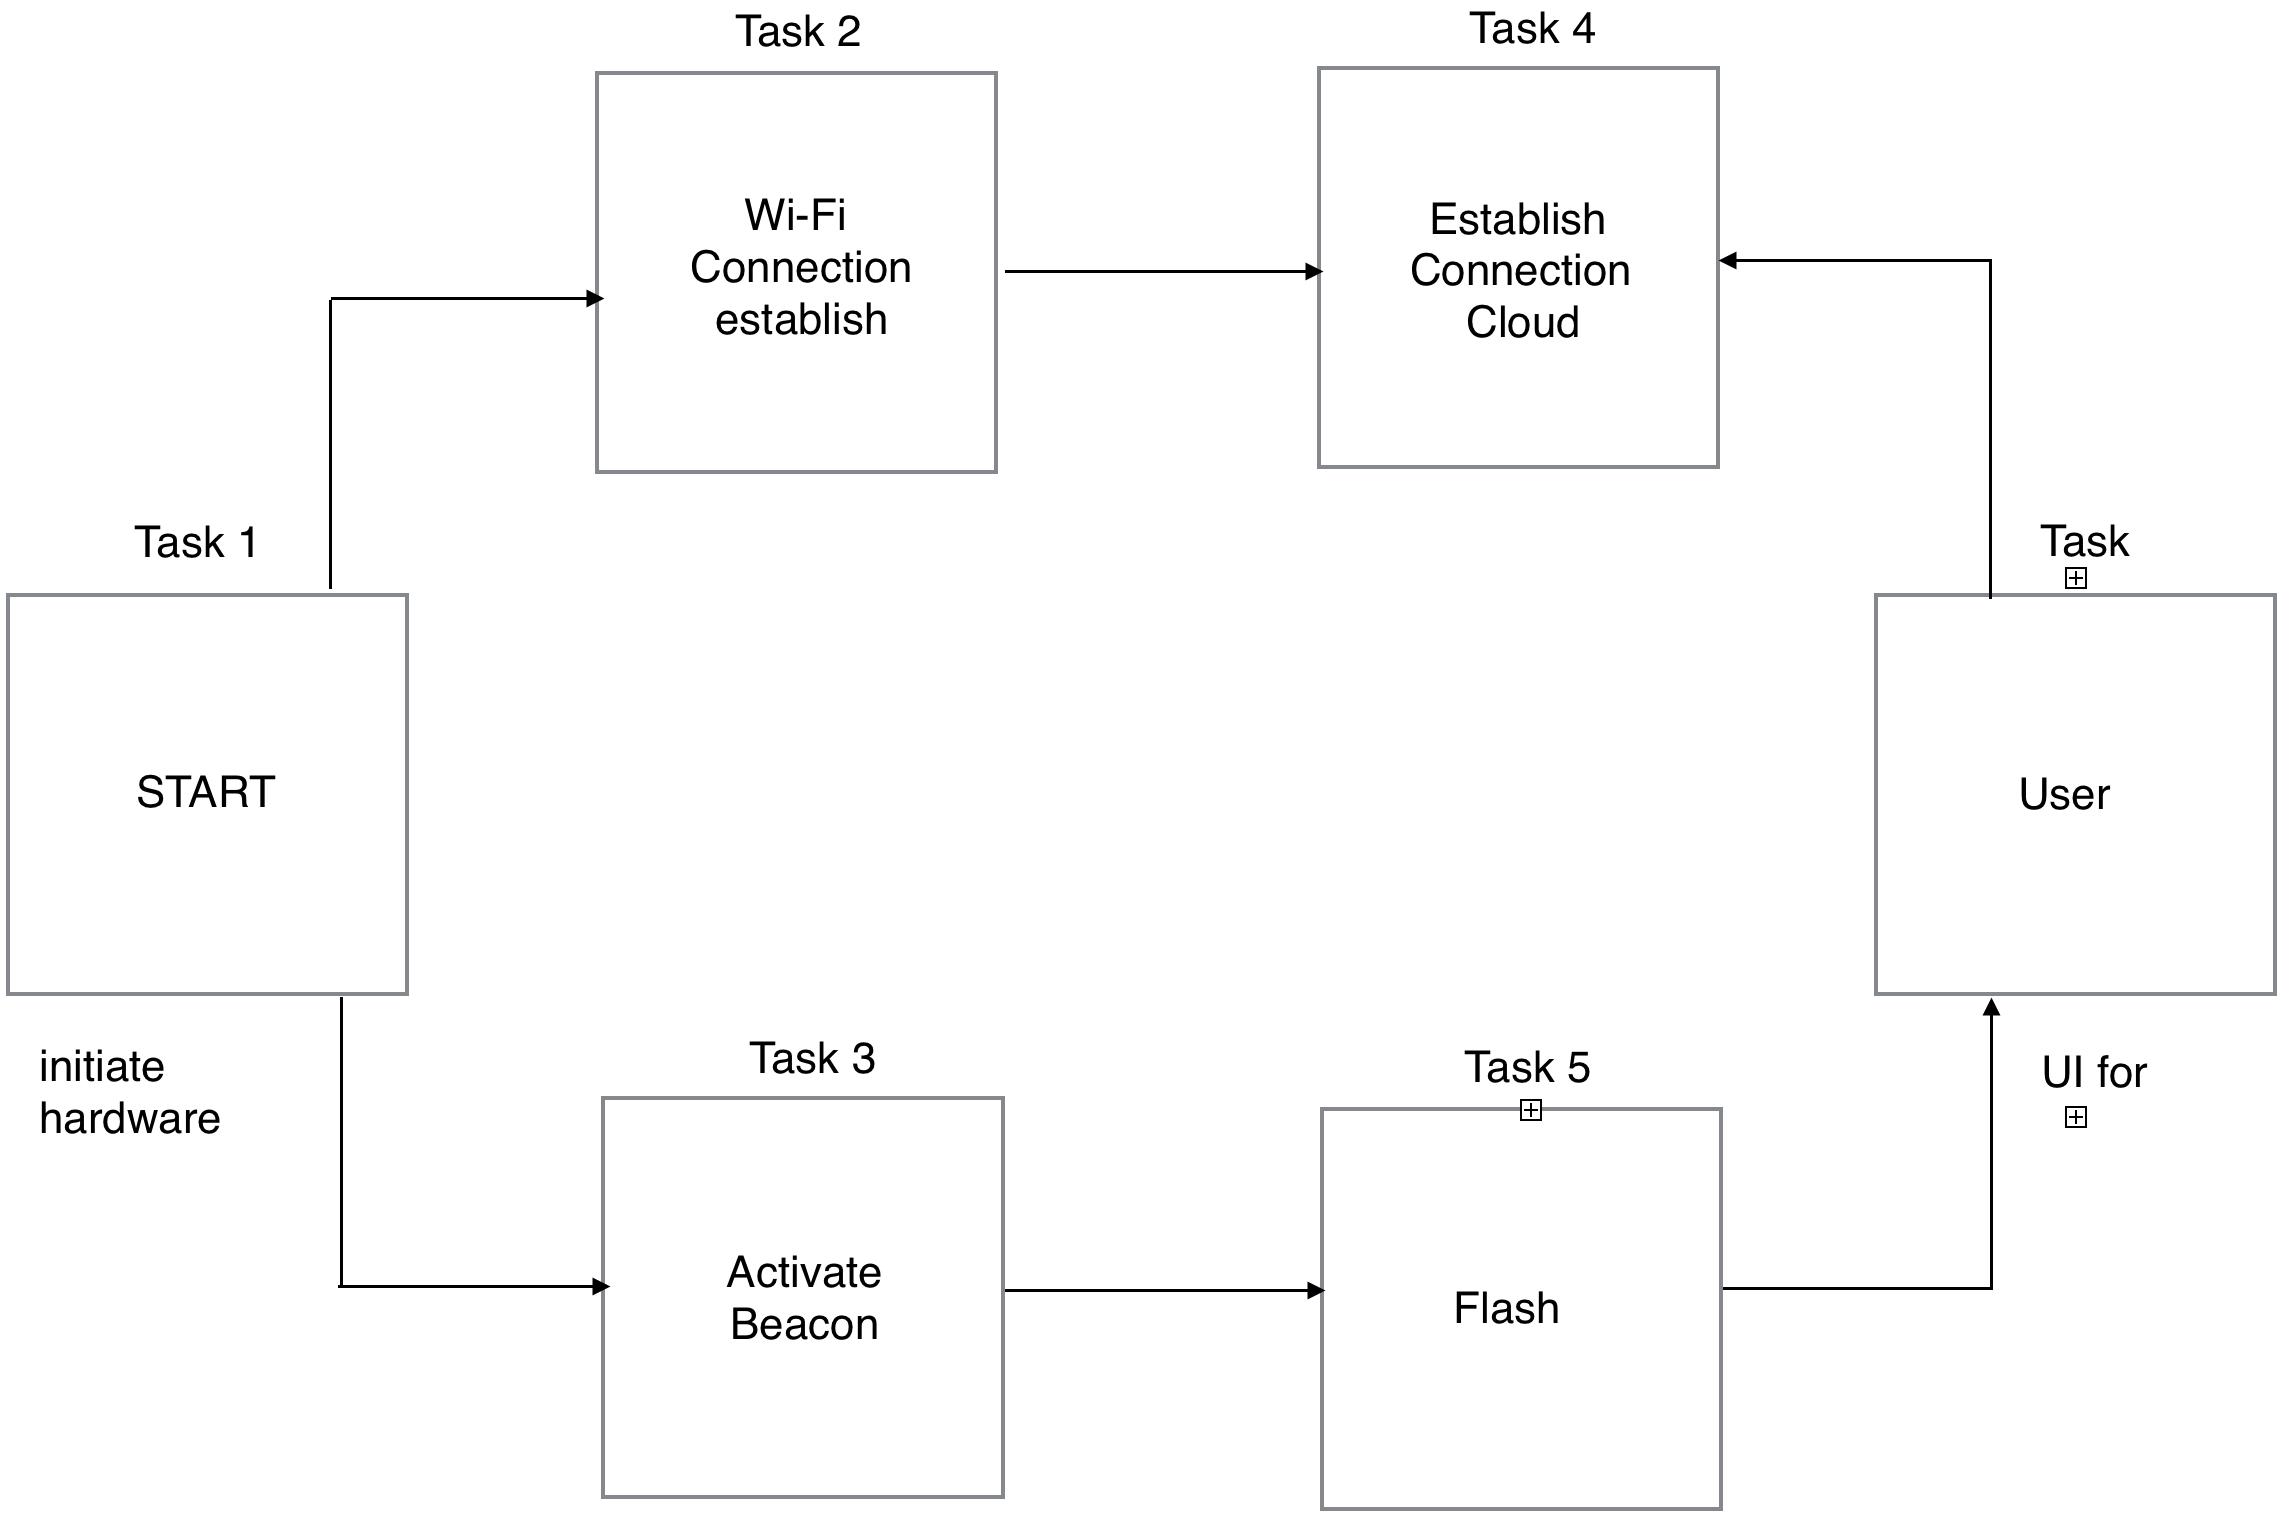
\includegraphics[height=250pt]{task.png}}
	  \caption{Activity diagram}
	  \label{fig:act-dig}
	\end{figure}
\end{center}  

\subsection{Timeline Chart}  

\begin{center}
	\begin{figure}[!htbp]
		\centering
		\fbox{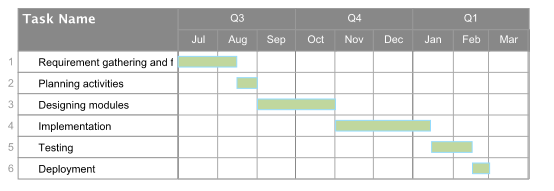
\includegraphics[height=150pt]{gantt.png}}
	  \caption{Activity diagram}
	  \label{fig:act-dig}
	\end{figure}
\end{center}  



 
\section{Team Organization}
College Guide - Prof A.R.Deshpande\\
Mentor - Mr. Anuj Deshpande \\

Our project guide helps us efficiently in the development of the project and helps us with our queries.
She also provides us with the much needed motivation.\\
Our mentor guides us through the project and helps us in defining a proper work flow of the project.\\ 

\subsection{Team structure}
The team structure for the project is identified.
Our project is divided into different smaller modules and the team works independently on  different modules.
We have three members in our group:\\
one working on the front end\\
one working on firmware\\
one working on cloud communication.\\

\subsection{Management reporting and communication}
Mechanisms for progress reporting and inter/intra team communication are identified as per assessment sheet and lab time table. 

\chapter{Software requirement specification  (SRS is to be prepared using relevant mathematics derived and software engg. Indicators in Annex A and B)}

\section{Introduction}
\subsection{Purpose and Scope of Document}
The purpose of SRS and what it covers is to be stated 

\subsection{Overview of responsibilities of Developer}
What all activities carried out by developer?
  
\section{Usage Scenario}
This section provides various usage scenarios for the system to be developed.  
 \subsection{User profiles}  
The profiles of all user categories are described here.(Actors and their Description)

\subsection{Use-cases}
All use-cases for the software are presented. Description of all main Use cases using use case template is to be provided.

\begin{table}[!htbp]
\begin{center}
%\def\arraystretch{1.5}
\def\arraystretch{1.5}
\begin{tabularx}{\textwidth}{| c | c | X | c | X |}
\hline
Sr No.	& Use Case	& Description	& Actors	& Assumptions \\
\hline
1& Use Case 1 & Description & Actors & Assumption \\
\hline
\end{tabularx}
\end{center}
\caption{Use Cases}
\label{tab:usecase}
\end{table}


\subsection{Use Case View}
Use Case Diagram. Example is given below
\begin{center}
	\begin{figure}[!htbp]
		\centering
		\fbox{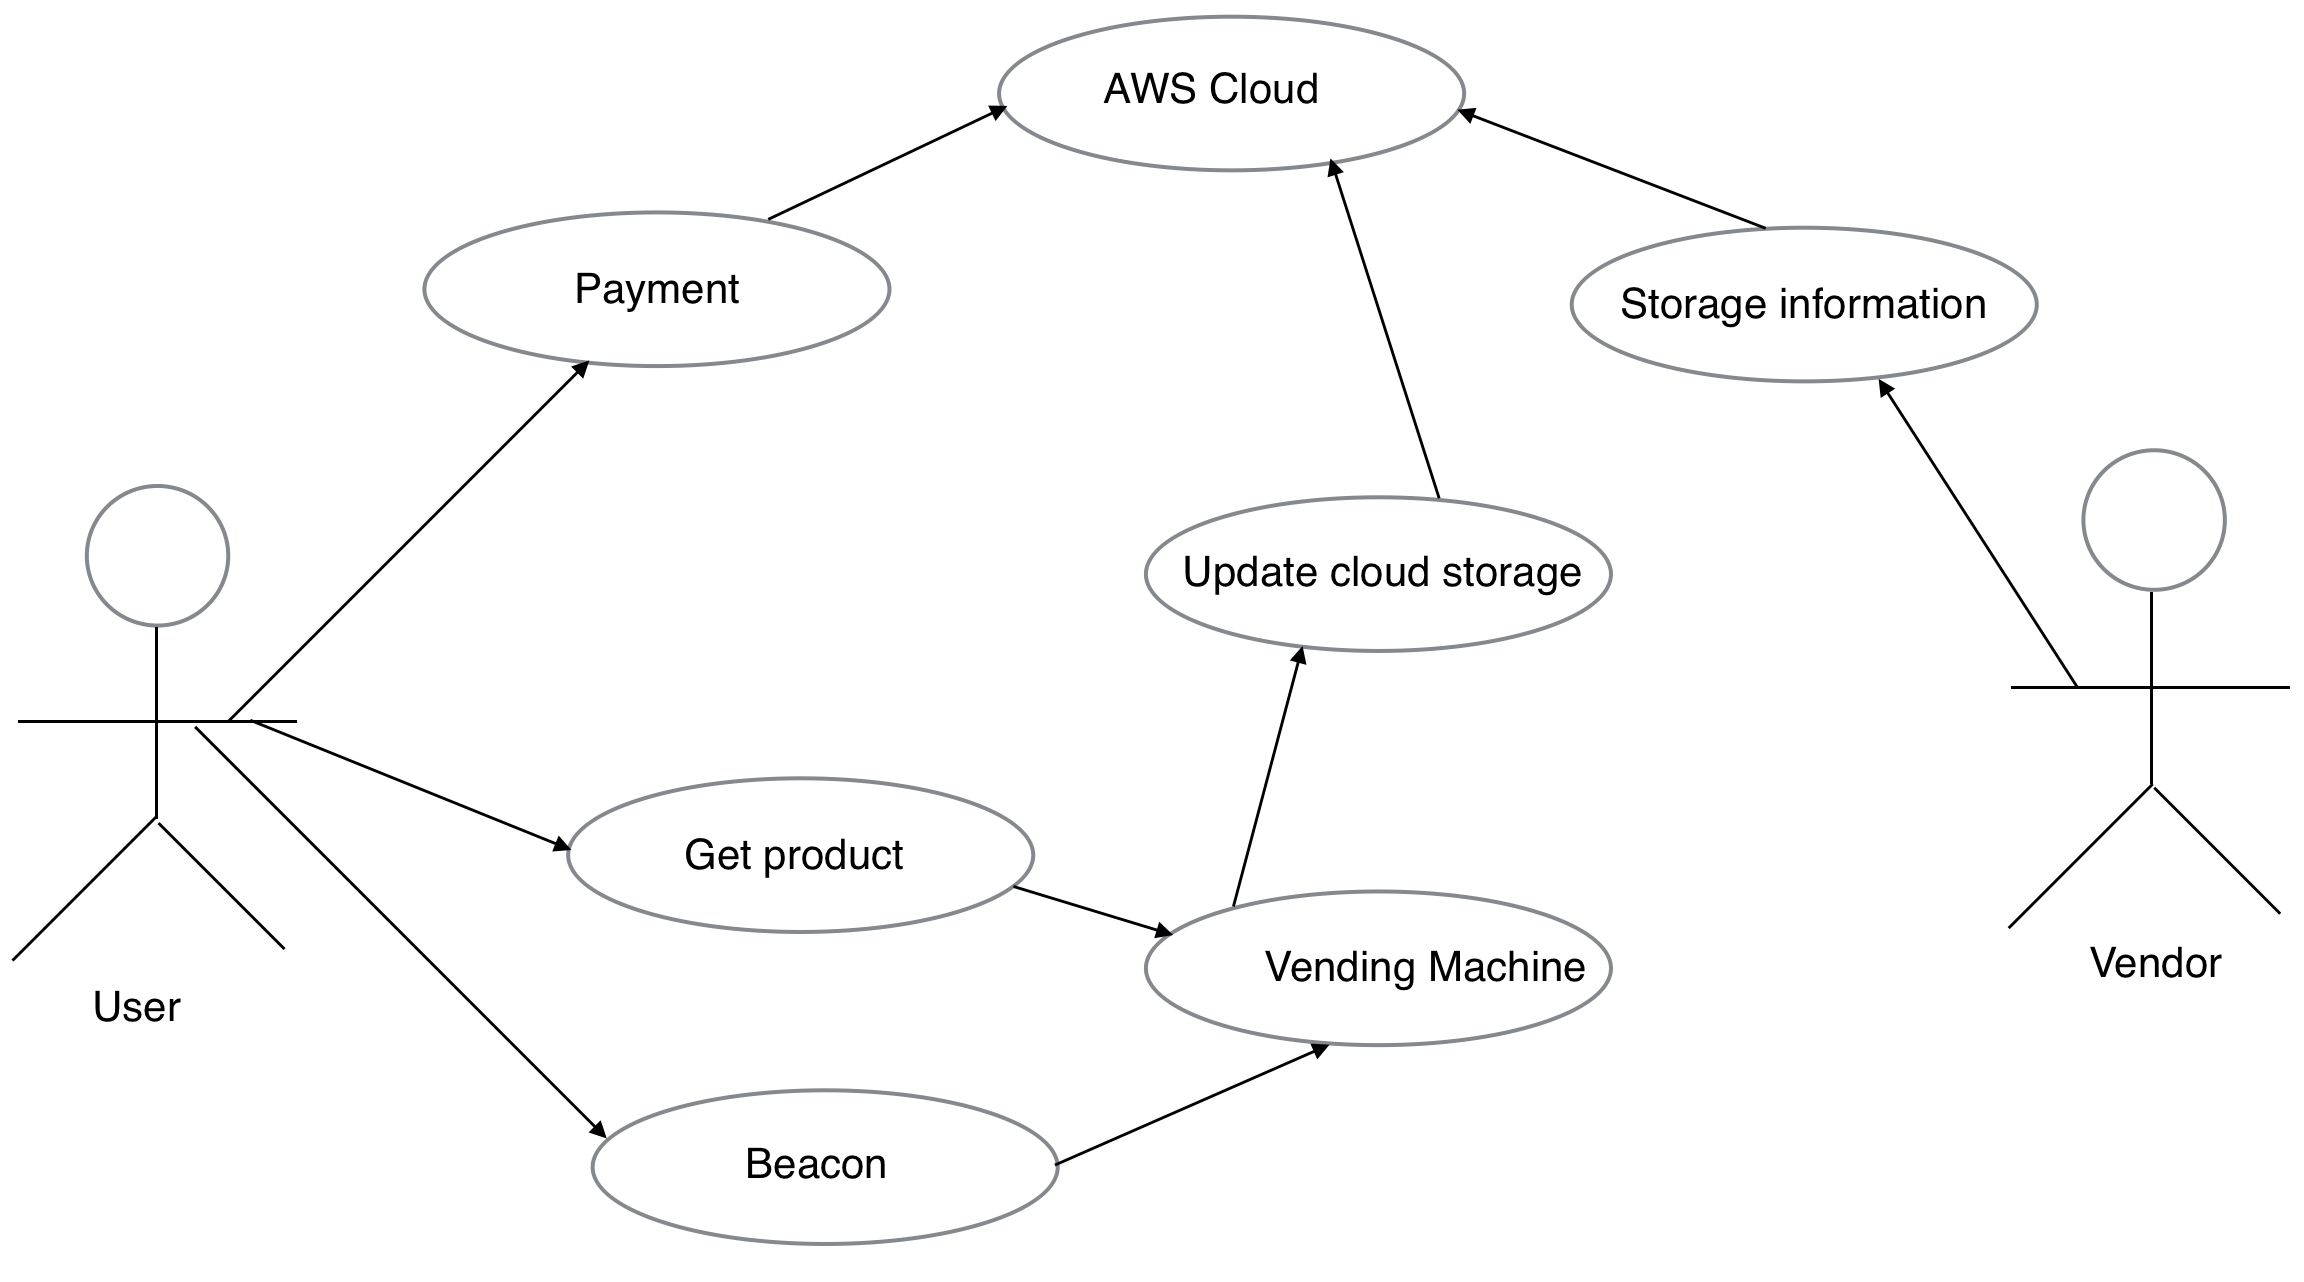
\includegraphics[width=\textwidth]{usecase.png}}
	  \caption{Use case diagram}
	  \label{fig:usecase}
	\end{figure}
\end{center}  

\section{Data Model and Description}  
\subsection{Data Description}  
Data objects that will be managed/manipulated by the software are described in this section. The database entities or files or data structures  required to be described. For data objects details can be given as below
\subsection{Data objects and Relationships}
  Data objects and their major attributes and relationships among data objects are described using an ERD- like form.

 
 
\section{Functional Model and Description}  
A description of each major software function, along with data flow (structured analysis) or class hierarchy (Analysis Class diagram with class description for object oriented system) is presented. 
\subsection{Data Flow Diagram}  
\subsubsection{Level 0 Data Flow Diagram}
\subsubsection{Level 1 Data Flow Diagram}
 
\subsection{Description of functions}  
A description of each software function is presented. A processing narrative for function n is presented.(Steps)/ Activity Diagrams. For Example Refer \ref{fig:act-dig}



\begin{center}
	\begin{figure}[!htbp]
		\centering
		\fbox{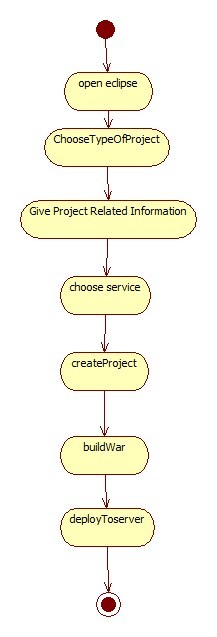
\includegraphics[height=430pt]{activity-dig.jpg}}
	  \caption{Activity diagram}
	  \label{fig:act-dig}
	\end{figure}
\end{center}  



 
\subsection{Activity Diagram:}
The Activity diagram represents the steps taken.

\subsection{Non Functional Requirements:}
Interface Requirements\\
Performance Requirements\\
Software quality attributes such as availability [ related to Reliability], modifiability [includes portability, reusability, scalability] , performance, security, testability and usability[includes self adaptability and user adaptability] \\

\subsection{State Diagram:}	
  State Transition Diagram\\

\begin{center}
	\begin{figure}[!htbp]
		\centering
		\fbox{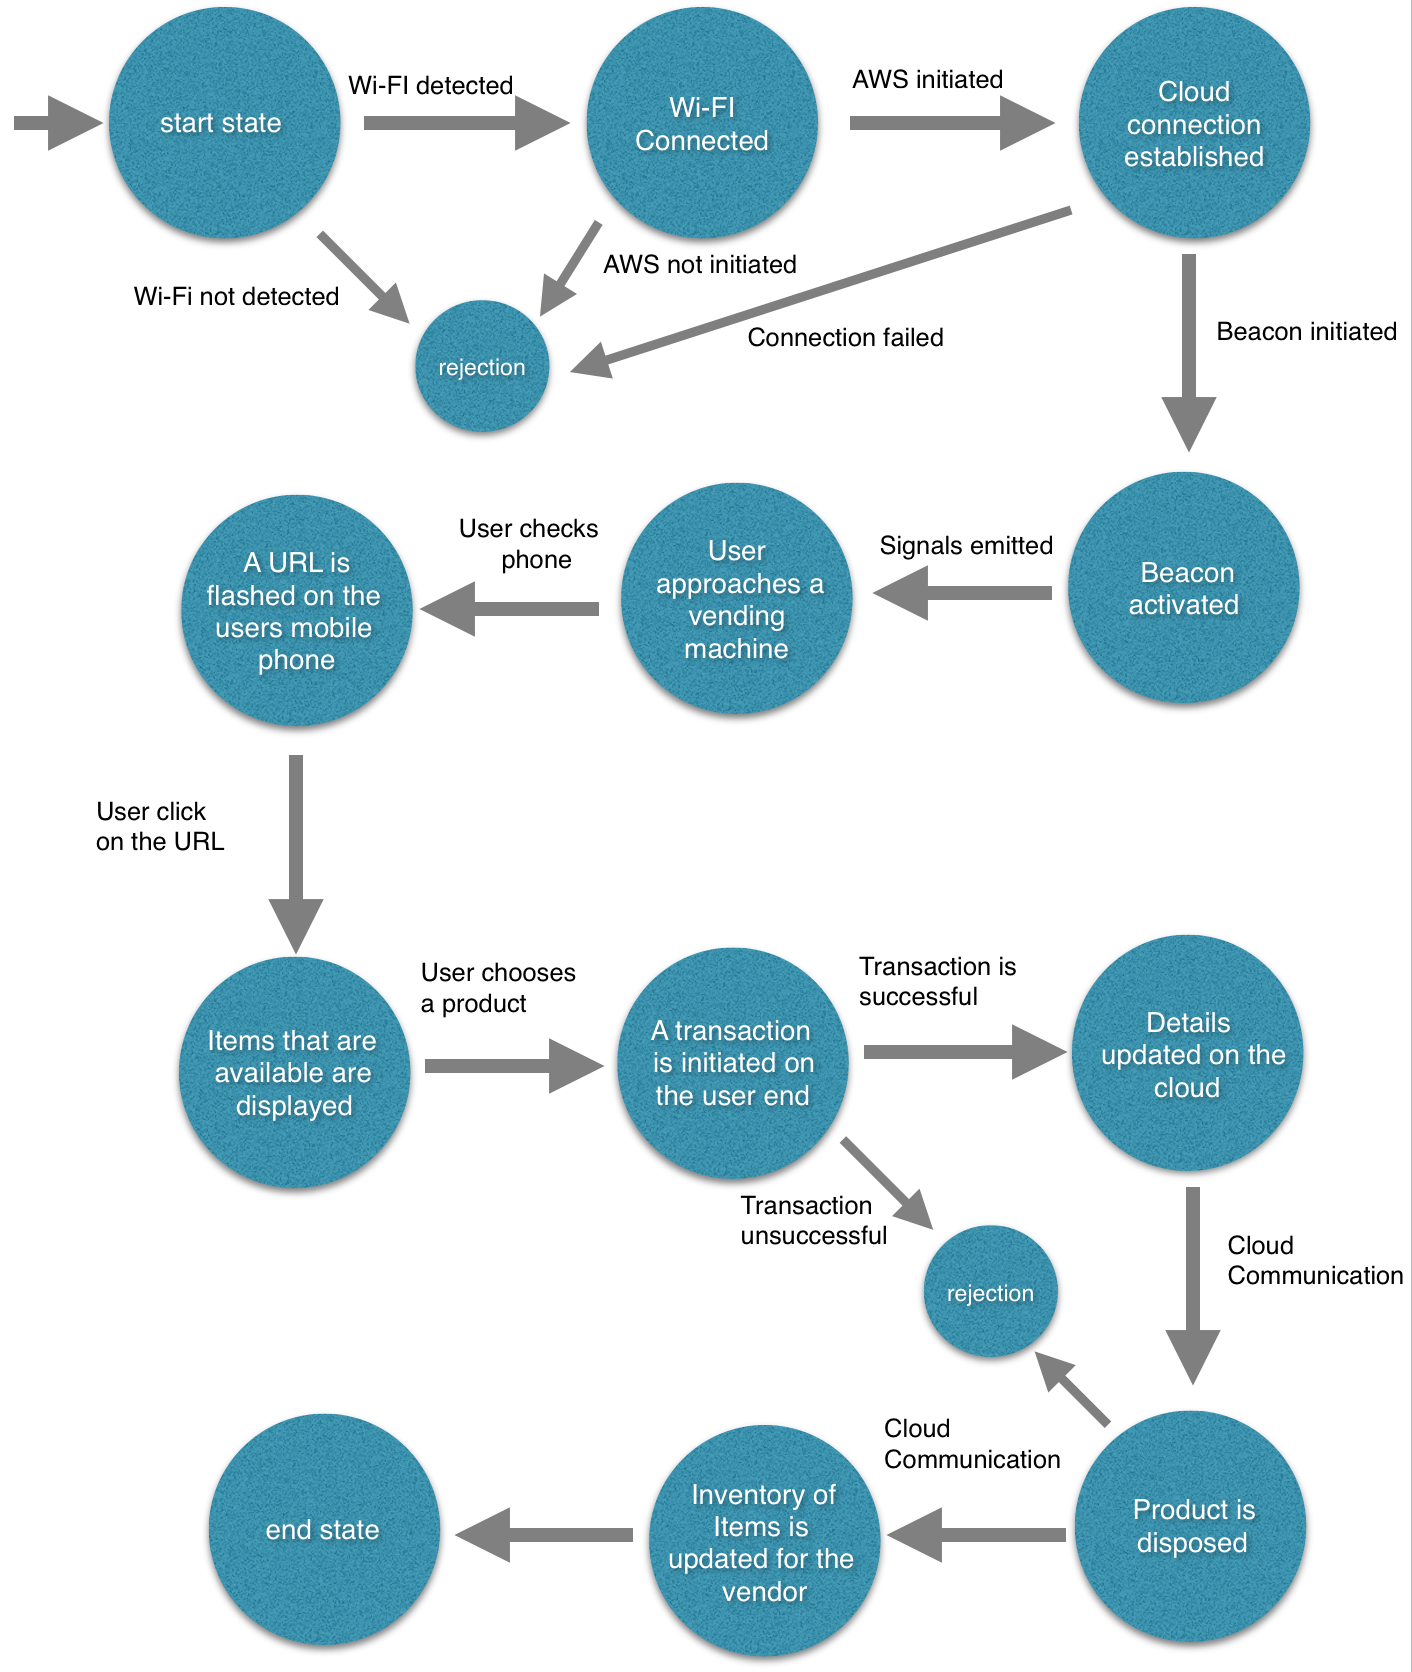
\includegraphics[width=450pt]{state.png}}
	  \caption{State transition diagram}
	  \label{fig:state-dig}
	\end{figure}
\end{center} 
\newpage
 \subsection{Design Constraints}	
Any design constraints that will impact the subsystem are noted.
 \subsection{Software Interface Description}	 
The software interface(s)to the outside world is(are) described.
The requirements for interfaces to other devices/systems/networks/human are stated.



\chapter{Detailed Design Document using Appendix A and B}
 \section{Introduction}  
This document specifies the design that is used to solve the problem of Product.  
\section{Architectural Design}  
	A description of the program architecture is presented. Subsystem design or Block diagram,Package Diagram,Deployment diagram with description is to be presented.

 
  \begin{center}
	\begin{figure}[!htbp]
		\centering
		\fbox{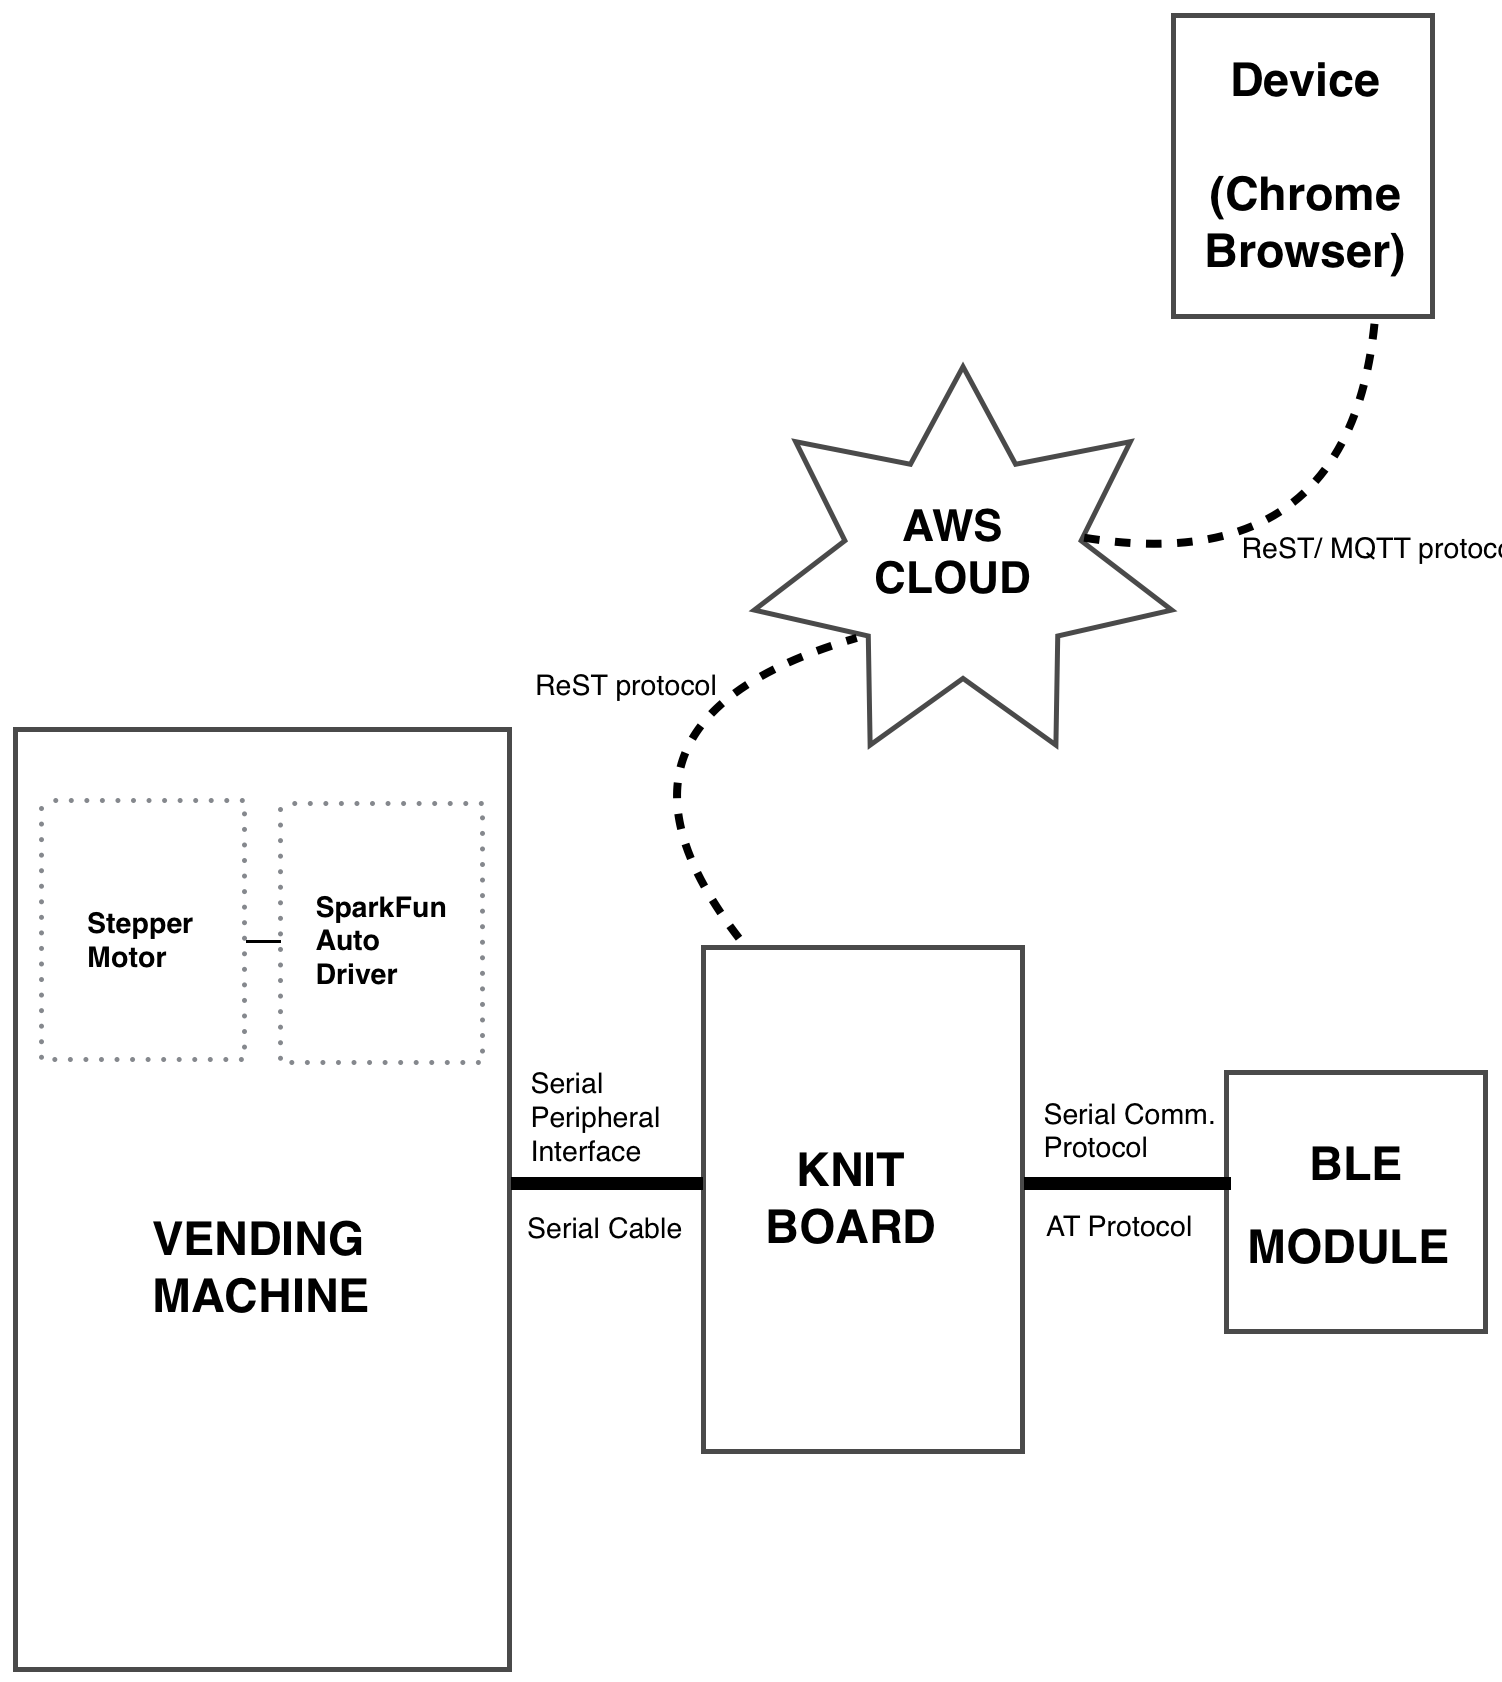
\includegraphics[width=\textwidth]{Arch.png}}
	  \caption{Architecture diagram}
	  \label{fig:arch-dig}
	\end{figure}
\end{center} 


\section{Data design (using Appendices A and B)}   
A description of all data structures including internal, global, and temporary data structures, database design (tables), file formats.
\subsection{Internal software data structure}
Data structures that are passed among components the software are described.
\subsection{Global data structure}
Data structured that are available to major portions of the architecture are described.
\subsection{Temporary data structure}
Files created for interim use are described.
\subsection{Database description}
Database(s) / Files created/used  as part of the application is(are) described.


\section{Compoent Design} 
Class diagrams, Interaction Diagrams, Algorithms. Description of each component description required.
\subsection{Class Diagram}
 \begin{center}
	\begin{figure}[!htbp]
		\centering
		\fbox{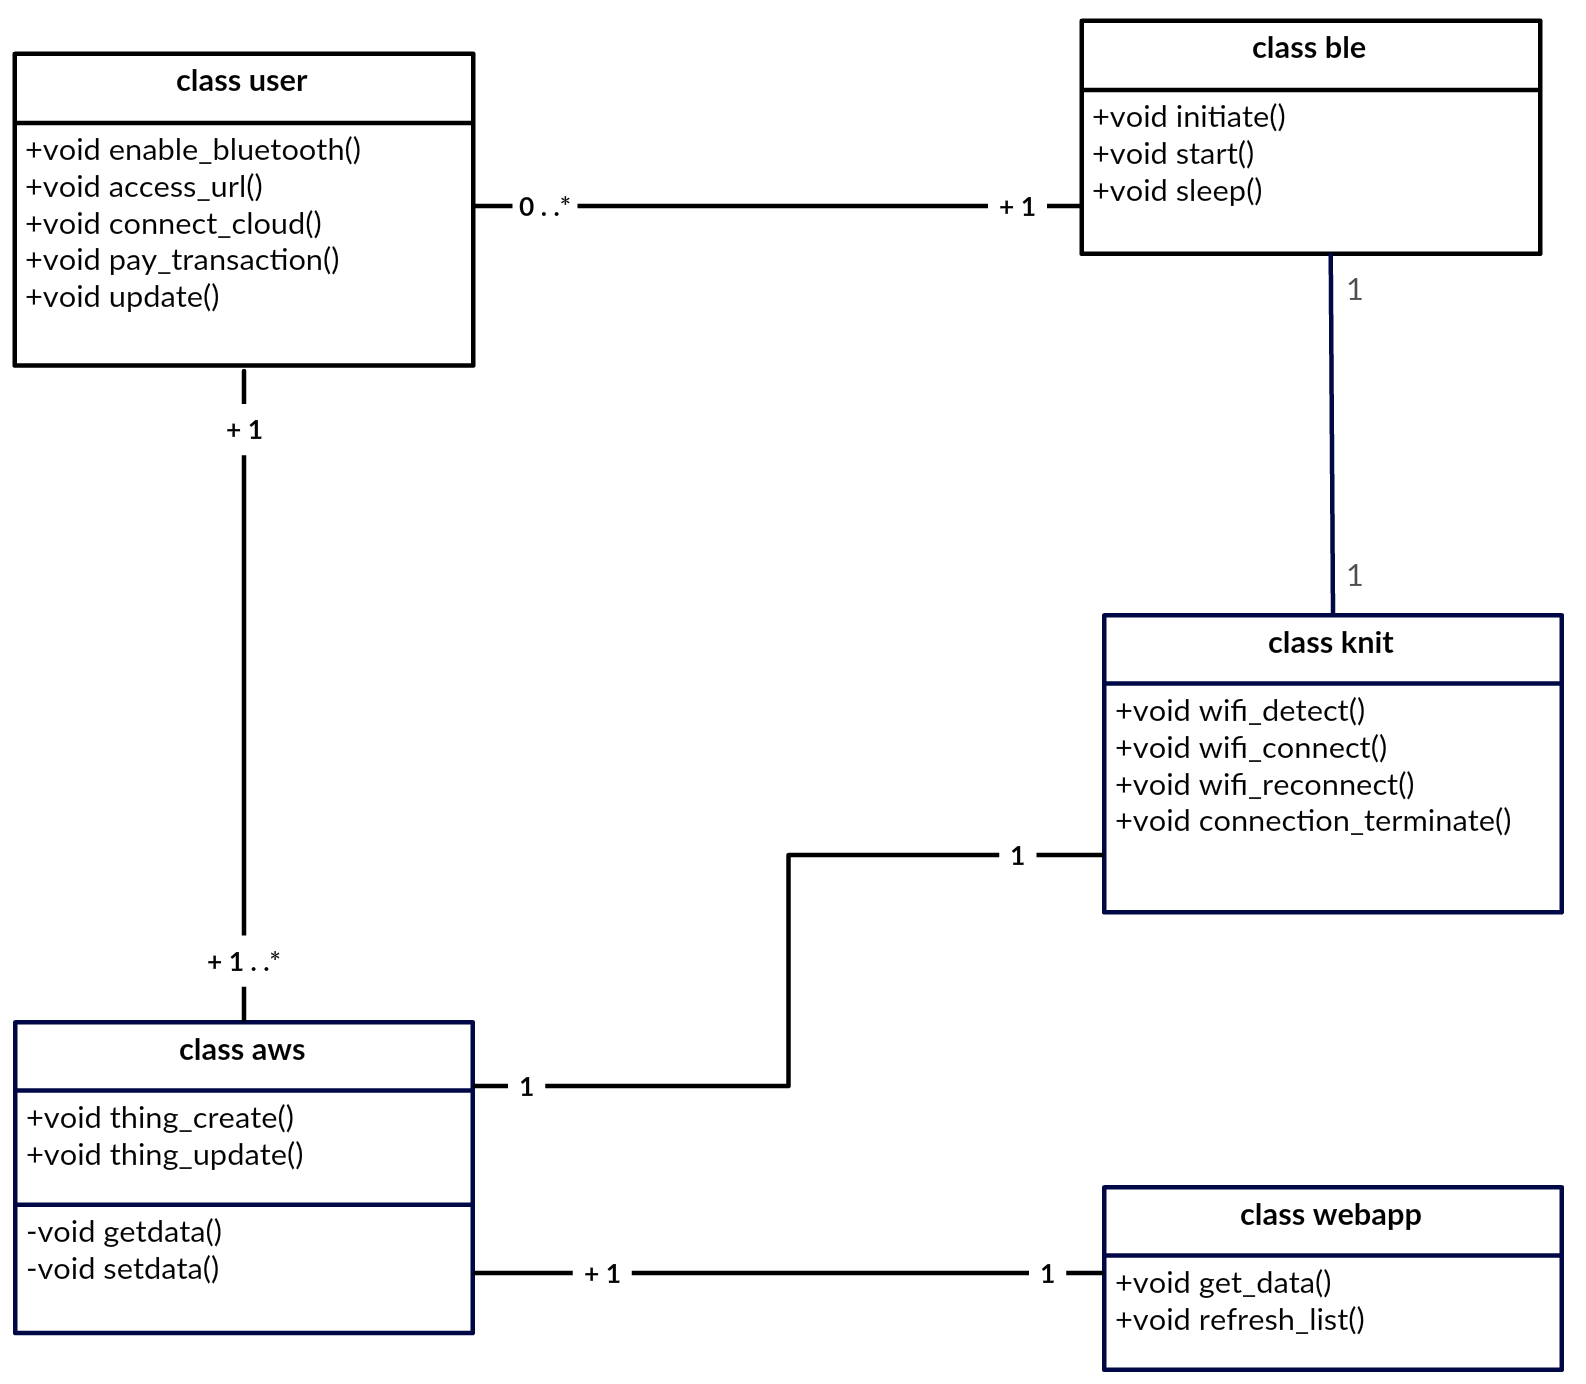
\includegraphics[width=450pt]{class.png}}
	  \caption{Class Diagram}
	  \label{fig:class-dig}
	\end{figure}
\end{center} 
 

\bibliographystyle{ieeetr}
\bibliography{biblo}
\begin{appendices}
\section{Summary and Conclusion}
We expect to learn web bluetooth technology and its applications .Also to learn how a actual product is launched and how to take care of the finished product delivery.
Steps in beginning of  this project from collecting the vendor requirements to take  care of the user test cases involved and then simulatng the environment to predict future risks and then applying Risk Management on it .


% \chapter{ALGORITHMIC DESIGN}
\chapter{Laboratory assignments on Project Analysis of Algorithmic Design}

To develop the problem under consideration and justify feasibilty using
concepts of knowledge canvas and IDEA Matrix.\\
Refer \cite{innovationbook} for IDEA Matrix and Knowledge canvas model. Case studies are given in this book. IDEA Matrix is represented in the following form. Knowledge canvas represents about identification  of opportunity for product. Feasibility is represented w.r.t. business perspective.\\ 

\begin{table}[!htbp]
\begin{center}
  \begin{tabular}{| c | c | c | c |}
\hline
 I & D & E & A \\ 
\hline
Increase & Drive & Educate & Accelerate \\
\hline
Improve & Deliver & Evaluate & Associate  \\
 \hline
Ignore & Decrease & Eliminate & Avoid \\
\hline
\end{tabular}
 \caption { IDEA Matrix }
 \label{tab:imatrix}
\end{center}
\end{table}

Project problem statement feasibility assessment using NP-Hard, NP-Complete or satisfy ability issues using modern algebra and/or relevant mathematical models.
 input x,output y, y=f(x)











\chapter{Laboratory assignments on Project Quality and Reliability Testing of Project Design}

It should include assignments such as\\
 Use of divide and conquer strategies to exploit distributed/parallel/concurrent processing of the above to identify object, morphisms, overloading in functions (if any), and functional relations and any other dependencies (as per requirements).\\
             It can include Venn diagram, state diagram, function relations, i/o relations; use this to derive objects, morphism, overloading\\

 Use of above to draw functional dependency graphs and relevant Software modeling methods, techniques including UML diagrams or other necessities using appropriate tools.
 \\
Testing of project problem statement using generated test data (using mathematical models, GUI, Function testing principles, if any) selection and appropriate use of testing tools, testing of UML diagram's reliability. Write also test cases [Black box testing] for each identified functions. \\
 Additional assignments by the guide. If project type as Entreprenaur, Refer \cite{ehr},\cite{mckinsey},\cite{mckinseyweb}, \cite{govwebsite}


\chapter{Project Planner}
\label{app:plan}
Using planner or alike project management tool.




\chapter{Reviewers Comments of Paper Submitted}
(At-least one technical paper must be submitted in Term-I on the project design in the
conferences/workshops in IITs, Central Universities or UoP Conferences or equivalent International Conferences Sponsored by IEEE/ACM)
\begin{enumerate}
\item Paper Title:
\item Name of the Conference/Journal where paper submitted :
\item Paper accepted/rejected : 
\item Review comments by reviewer :
\item Corrective actions if any :  

\end{enumerate}

\chapter{Plagiarism Report}
Plagiarism report


\end{appendices}


\end{document}
